\let\negmedspace\undefined
\let\negthickspace\undefined
\documentclass[journal]{IEEEtran}
\usepackage[a5paper, margin=10mm, onecolumn]{geometry}
%\usepackage{lmodern} % Ensure lmodern is loaded for pdflatex
\usepackage{tfrupee} % Include tfrupee package

\setlength{\headheight}{1cm} % Set the height of the header box
\setlength{\headsep}{0mm}     % Set the distance between the header box and the top of the text

\usepackage{gvv-book}
\usepackage{gvv}
\usepackage{cite}
\usepackage{amsmath,amssymb,amsfonts,amsthm}
\usepackage{algorithmic}
\usepackage{graphicx}
\usepackage{textcomp}
\usepackage{xcolor}
\usepackage{txfonts}
\usepackage{listings}
\usepackage{enumitem}
\usepackage{mathtools}
\usepackage{gensymb}
\usepackage{comment}
\usepackage[breaklinks=true]{hyperref}
\usepackage{tkz-euclide} 
\usepackage{listings}
% \usepackage{gvv}                                        
\def\inputGnumericTable{}                                 
\usepackage[latin1]{inputenc}                                
\usepackage{color}                                            
\usepackage{array}                                            
\usepackage{longtable}                                       
\usepackage{calc}                                             
\usepackage{multirow}                                         
\usepackage{hhline}                                           
\usepackage{ifthen}                                           
\usepackage{lscape}
\begin{document}

\bibliographystyle{IEEEtran}
\vspace{3cm}

\title{1.1.9.28}
\author{EE24BTECH11059 - Yellanki Siddhanth
}
% \maketitle
% \newpage
% \bigskip
{\let\newpage\relax\maketitle}

\renewcommand{\thefigure}{\theenumi}
\renewcommand{\thetable}{\theenumi}
\setlength{\intextsep}{10pt} % Space between text and floats


\numberwithin{equation}{enumi}
\numberwithin{figure}{enumi}
\renewcommand{\thetable}{\theenumi}


\textbf{Question}:\\
If $\vec{A}$ and $\vec{B}$ are the points $\brak{-6, 7}$ and $\brak{-1, -5}$ respectively, then the distance $\vec{2AB}$ is
equal to
\\ \textbf{Solution: }\\
    \begin{table}[h!]    
      \centering
      

      \caption{}
    \end{table}\\
    To calculate the distance AB,
    \begin{align}
        \vec{A}-\vec{B} = \myvec{-6 \\ 7} - \myvec{-1 \\ -5} = \myvec{-5 \\ 12}\label{eq1.1.9.28.1}
    \end{align}
    \begin{align}
    	\abs{\abs{\vec{A}-\vec{B}}}^2 = \brak{\vec{A}-\vec{B}}^\top \brak{\vec{A}-\vec{B}}\label{eq1.1.9.28.2}
    \end{align}
    \begin{align}
		 \brak{\vec{A}-\vec{B}}^\top \brak{\vec{A}-\vec{B}} = \myvec{-5 & 12}\myvec{-5 \\ 12} = 169\label{eq1.1.9.28.3}
	\end{align}
	Thus the distance AB is,
    \begin{align}
	\abs{\abs{\vec{A}-\vec{B}}} = \sqrt{169}= 13 \label{eq1.1.9.28.4}
	\end{align}
	$\therefore$ Required value is:
	\begin{align}
		\vec{2AB} = 26
	\end{align}
    \begin{figure}[h]
        \centering
       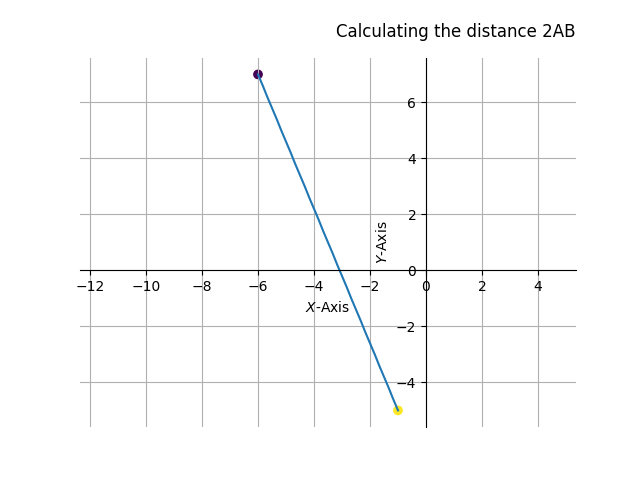
\includegraphics[width=0.7\linewidth]{figs/fig1.png}
       \caption{}
       \label{graph}
    \end{figure}



\end{document}  







